% !TEX encoding = UTF-8 Unicode
%%%%%%%%%%%%%%%%%%%%%%%%%%%%%%%%%%%%%%%%%
% Beamer Presentation
% LaTeX Template
% Version 1.0 (10/11/12)
%
% This template has been downloaded from:
% http://www.LaTeXTemplates.com
%
% License:
% CC BY-NC-SA 3.0 (http://creativecommons.org/licenses/by-nc-sa/3.0/)
%
%%%%%%%%%%%%%%%%%%%%%%%%%%%%%%%%%%%%%%%%%

%----------------------------------------------------------------------------------------
%	PACKAGES AND THEMES
%----------------------------------------------------------------------------------------

\documentclass{beamer}

\mode<presentation> {

% The Beamer class comes with a number of default slide themes
% which change the colors and layouts of slides. Below this is a list
% of all the themes, uncomment each in turn to see what they look like.

%\usetheme{default}
%\usetheme{AnnArbor}
%\usetheme{Antibes}
%\usetheme{Bergen}
%\usetheme{Berkeley}
%\usetheme{Berlin}
%\usetheme{Boadilla}
%\usetheme{CambridgeUS}
%\usetheme{Copenhagen}
%\usetheme{Darmstadt}
%\usetheme{Dresden}
%\usetheme{Frankfurt}
%\usetheme{Goettingen}
%\usetheme{Hannover}
%\usetheme{Ilmenau}
%\usetheme{JuanLesPins}
%\usetheme{Luebeck}
\usetheme{Madrid}
%\usetheme{Malmoe}
%\usetheme{Marburg}
%\usetheme{Montpellier}
%\usetheme{PaloAlto}
%\usetheme{Pittsburgh}
%\usetheme{Rochester}
%\usetheme{Singapore}
%\usetheme{Szeged}
%\usetheme{Warsaw}

% As well as themes, the Beamer class has a number of color themes
% for any slide theme. Uncomment each of these in turn to see how it
% changes the colors of your current slide theme.

%\usecolortheme{albatross}
%\usecolortheme{beaver}
%\usecolortheme{beetle}
%\usecolortheme{crane}
%\usecolortheme{dolphin}
%\usecolortheme{dove}
%\usecolortheme{fly}
%\usecolortheme{lily}
%\usecolortheme{orchid}
%\usecolortheme{rose}
%\usecolortheme{seagull}
%\usecolortheme{seahorse}
%\usecolortheme{whale}
%\usecolortheme{wolverine}

%\setbeamertemplate{footline} % To remove the footer line in all slides uncomment this line
%\setbeamertemplate{footline}[page number] % To replace the footer line in all slides with a simple slide count uncomment this line

%\setbeamertemplate{navigation symbols}{} % To remove the navigation symbols from the bottom of all slides uncomment this line
}

\usepackage{graphicx} % Allows including images
\usepackage{booktabs} % Allows the use of \toprule, \midrule and \bottomrule in tables
\usepackage{xeCJK}
\usepackage{color}
\usepackage{listings}
\lstset{numbers=left}
\usepackage{tikz}


%----------------------------------------------------------------------------------------
%	TITLE PAGE
%----------------------------------------------------------------------------------------

\title[Process]{Process} % The short title appears at the bottom of every slide, the full title is only on the title page

\author{张海宁} % Your name
\institute[计算机科学与技术学院] % Your institution as it will appear on the bottom of every slide, may be shorthand to save space
{
贵州大学 \\ % Your institution for the title page
\medskip
\textit{hnzhang1@gzu.edu.cn} % Your email address
}
\date{\today} % Date, can be changed to a custom date

\begin{document}

\begin{frame}
\titlepage % Print the title page as the first slide
\end{frame}

\begin{frame}
\frametitle{Overview} % Table of contents slide, comment this block out to remove it
\tableofcontents % Throughout your presentation, if you choose to use \section{} and \subsection{} commands, these will automatically be printed on this slide as an overview of your presentation
\end{frame}

%----------------------------------------------------------------------------------------
%	PRESENTATION SLIDES
%----------------------------------------------------------------------------------------
\section{Process}
\begin{frame}
\Huge{\centerline{Process}}
\end{frame}
\subsection{What is a Process}
\begin{frame}
\Huge{\centerline{What is a Process}}
\end{frame}
\begin{frame}{Process}
\begin{itemize}
\item
A process is \textcolor{red}{a program that is running}.
\item
A process is running consists of program code, data, variables (occupying system memory), open files (file descriptors), and an environment.
\end{itemize}
\emph{Typically, a Linux system will share code and system libraries among processes so that there’s only one copy of the code in memory at any one time.}
\end{frame}
\subsection{Process Structure}
\begin{frame}{Process Structure}
\begin{figure}

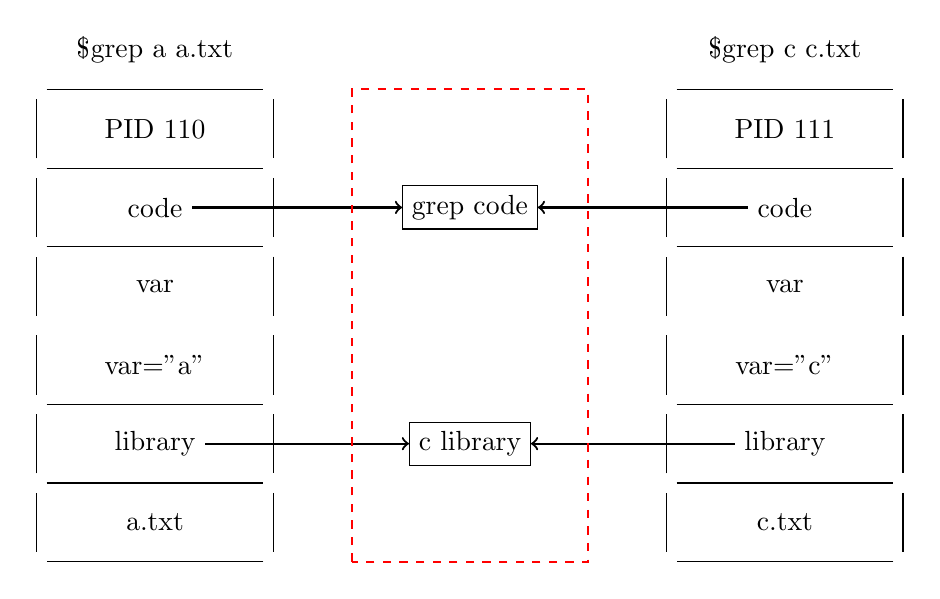
\begin{tikzpicture}
\node (a) at (0,0) {};
\node (b) at (0,1) {};
\node (c) at (0,2) {};
\node (d) at (0,3) {};
\node (e) at (0,4) {};
\node (f) at (0,5) {};
\node (g) at (0,6) {};
\node (h) at (3,6) {};
\node (i) at (3,5) {};
\node (j) at (3,4) {};
\node (k) at (3,3) {};
\node (l) at (3,2) {};
\node (m) at (3,1) {};
\node (n) at (3,0) {};
\draw (a) -- (b) -- (c)--(d)--(e)--(f)--(g)--(h)--(i)--(j)--(k)--(l)--(m)--(n)--(a);
\draw (b)--(m);
\draw (c)--(l);
%\draw (d)--(k);
\draw (e)--(j);
\draw (f)--(i);
\node (5) at(1.5,0.5) {a.txt};
\node (4) at(1.5,1.5) {library};
\node (3) at(1.5,2.5) {var="a"};
\node (2) at(1.5,3.5) {var};
\node (1) at(1.5,4.5) {code};
\node (0) at(1.5,5.5) {PID 110};
\node(00) at(1.5,6.5) {\$grep a a.txt};

\node (aa) at (8,0) {};
\node (bb) at (8,1) {};
\node (cc) at (8,2) {};
\node (dd) at (8,3) {};
\node (ee) at (8,4) {};
\node (ff) at (8,5) {};
\node (gg) at (8,6) {};
\node (hh) at (11,6) {};
\node (ii) at (11,5) {};
\node (jj) at (11,4) {};
\node (kk) at (11,3) {};
\node (ll) at (11,2) {};
\node (mm) at (11,1) {};
\node (nn) at (11,0) {};
\draw (aa) -- (bb) -- (cc)--(dd)--(ee)--(ff)--(gg)--(hh)--(ii)--(jj)--(kk)--(ll)--(mm)--(nn)--(aa);
\draw (bb)--(mm);
\draw (cc)--(ll);
%\draw (d)--(k);
\draw (ee)--(jj);
\draw (ff)--(ii);
\node (55) at(9.5,0.5) {c.txt};
\node (44) at(9.5,1.5) {library};
\node (33) at(9.5,2.5) {var="c"};
\node (22) at(9.5,3.5) {var};
\node (11) at(9.5,4.5) {code};
\node (000) at(9.5,5.5) {PID 111};
\node(0000) at(9.5,6.5) {\$grep c c.txt};
\node [draw,rectangle] (c) at(5.5,1.5) {c library};
\node [draw,rectangle] (g) at(5.5,4.5) {grep code};
\draw [->,thick] (4)--(c);
\draw [->,thick] (44)--(c);
\draw [->,thick] (1)--(g);
\draw [->,thick] (11)--(g);
\draw [red,dashed,thick] (4,0) rectangle (7,6);
\end{tikzpicture}
\caption{process structure}
\label{processstruct}
\end{figure}
\end{frame}
\begin{frame}{分析}
Figure \ref{processstruct} 显示了操作系统如何安排两个同时运行的grep程序(一种可能的状态)。从中我们可以看出:
\begin{enumerate}
\item
Each process is allocated a unique number, called a \textcolor{red}{process identifier or PID}(This is usually a positive integer between 2 and 32,768, The number 0/1 is typically reserved for the special init process, which manages other processes). 
\item
The \textcolor{red}{code of grep} was loaded into memory as read-only and was \textcolor{red}{shared} by the two processes. The \textcolor{red}{system library} worked the same way as the grep code.
\item
A process has its \textcolor{red}{own stack space}, used for local variables in functions and for controlling function calls and returns. It also has its \textcolor{red}{own environment space}, containing environment variables.
\end{enumerate}
\end{frame}
\begin{frame}{The Process Table}
The Linux \textcolor{red}{process table} is like a data structure describing all of the processes that are currently loaded with, for example, their PID, status, and command string, the sort of information output by \textcolor{red}{ps}. 
\end{frame}
\begin{frame}[fragile]{ps I}
\label{proclist}
The ps utility displays a header line, followed by lines containing information about all of your processes.
\begin{block}{list processes}
\begin{verbatim}
$ ps -f -u zhanghaining
UID        PID  PPID  C STIME TTY        TIME CMD
zhangha+ 25020 25015  0 13:18 ?    00:00:00 sshd: zhn@pts/3
zhangha+ 25021 25020  0 13:18 pts/3  00:00:00 -bash
zhangha+ 25201 25021  0 13:45 pts/3  00:00:00 ps -f -u zhn
\end{verbatim}
\end{block}
\end{frame}
\begin{frame}{分析}
\begin{itemize}
\item
The PPID field of ps output indicates the parent process ID, the PID of either the process that caused this
process to start or, if that process is no longer running, init (PID 1).
\item
TTY column shows which terminal the process was started from
\item
TIME gives the CPU time used so far
\item
the CMD column shows the command used to start the process
\end{itemize}
\end{frame}
\begin{frame}[fragile]{ps II}
we will show how to view the status of a process.
\begin{block}{status of process}
\begin{verbatim}
$ ps ax
 PID TTY      STAT   TIME COMMAND
25020 ?        S      0:00 sshd: zhanghaining@pts/3
25021 pts/3    Ss     0:00 -bash
25109 ?        S      0:00 [kworker/5:2]
25114 ?        S      0:00 [kworker/2:0]
25155 ?        S      0:00 [kworker/5:0]
25179 pts/3    R+     0:00 ps ax
\end{verbatim}
\end{block}
\end{frame}
\begin{frame}{ps III}
\begin{block}{status}
\begin{table}
\begin{tabular}{lp{20em}}
\toprule
\textbf{STAT Code}&\textbf{Description}\\
\midrule
S&Sleeping. Usually waiting for an event to occur, such as a signal or input to become available.\\
R&Running. Strictly speaking, “runnable,” that is, on the run queue either executing or about to run.\\
Z&Defunct or “zombie” process.\\
+&Process is in the foreground process group.\\
<&High priority task.\\
\bottomrule
\end{tabular}
\caption{some status}
\end{table}
\end{block}
\end{frame}
\subsection{Starting New Process}
\begin{frame}
\Huge{\centerline{Starting New Process}}
\end{frame}
\begin{frame}[fragile]{system I}
We can cause a program to run from inside another program and thereby create a new process by using the \textcolor{red}{system} library function.
\begin{block}{system}
\begin{verbatim}
#include <stdlib.h>
int system (const char *string);

\end{verbatim}
\end{block}
\begin{block}{man 3 system}
system -- pass a command to the shell
\end{block}
system returns 127 if a shell can’t be started to run the command and -1 if
another error occurs. Otherwise, system returns the exit code of the command.
\end{frame}

\begin{frame}[fragile]{system II}
use \textcolor{red}{system} to write a program to run ps.
\begin{block}{system}
\begin{verbatim}
$ cat system1.c
#include<stdlib.h>
#include<stdio.h>

int main(){
 printf("running ps with my program.\n");
 int i = system("ps x");
 //int i = system("ps x &");
 printf("Done. And the return code is:%d.\n",i);
 exit(0);
}
\end{verbatim}
\end{block}

\end{frame}
\begin{frame}{sytem III}
In general, using system is a far from ideal way to start other processes, because it invokes the desired program using a shell. 
\begin{enumerate}
\item
inefficient

a shell must be started before the program is stared.
\item
between shells

quite dependent on the installation for the shell and environment that are used.
\end{enumerate}\end{frame}

\begin{frame}{exec}
An exec function \textcolor{red}{replaces the current process} with a new process specified by the path or file argument.

The exec functions are more efficient than system because \textcolor{red}{the original program will no longer be running} after the new one is started.

\end{frame}
\begin{frame}{exec family}
execl, execle, execlp, execv, execvp -- execute a file
\begin{enumerate}
\item
execl, execle,execlp

参数可变,长度不固定
\item
 execv, execvp
 
 参数不可变,长度固定
\end{enumerate}
\end{frame}
\begin{frame}[fragile]{execl, execle,execlp}
\begin{block}{}
\begin{verbatim}
#include <unistd.h>
int
execl(const char *path, const char *arg0, ... , 
  (char *)0);

int
execle(const char *path, const char *arg0, ... , 
  (char *)0, char *const envp[] );

int
execlp(const char *file, const char *arg0, ... , 
  (char *)0);
\end{verbatim}
\end{block}
\end{frame}
\begin{frame}[fragile]{ execv, execvp}
\begin{block}{}
\begin{verbatim}

#include <unistd.h>
int
execv(const char *path, char *const argv[]);

int
execvp(const char *file, char *const argv[]);
\end{verbatim}
\end{block}
\end{frame}
\begin{frame}[fragile]{参数说明}
对于exec函数来说,第一个参数是要执行程序的路径名;其次的参数是要执行程序的文件名;然后是其他参数,有一点要注意的是,参数列表要以一个空指针结尾。
\begin{block}{例子}
\begin{verbatim}
$ cat execlp.c 
#include<unistd.h>
#include<stdio.h>
#include<stdlib.h>
int main(){
printf("Running ps with execlp:\n");
//execlp("ps","ps","ax",0);
execlp("/Users/hainingzhang/linux/system1","system1",0);
printf("Done.\n");
exit(0);
}

\end{verbatim}
\end{block}
\end{frame}
\begin{frame}{exec启动程序的特点}
\begin{itemize}
\item
exec启动的新程序会替换掉旧的程序,即原程序会消失,原程序exec之后的语句也不会再执行。
\item
exec启动的新程序会继承原有程序的许多特征,包括文件描述符等。
\end{itemize}
\end{frame}
\begin{frame}{复制一个进程镜像}
如果想使用一个进程同时运行多个程序,使用exec是不可以的,因为它会替换掉原有进程。

为了达到这个目的,可以使用多线程,或者fork系统调用+exec函数。

fork会创建一个跟原始进程几乎一样的进程,但是这个新进程拥有自己独立的pid和地址空间,可以认为是两个不同的进程,然后在新的进程里执行其他操作。
\begin{block}{fork}
 fork -- create a new process

\#include <unistd.h>

pid\_t   fork(void);
\end{block}

\begin{enumerate}
\item
fork() returns a value of \textcolor{red}{0 to the child process}
\item
returns the \textcolor{red}{process ID of the child} process to the \textcolor{red}{parent} process
\item
Otherwise, a value of -1 is returned to the parent process.
\end{enumerate}
\end{frame}
\begin{frame}{fork图示}
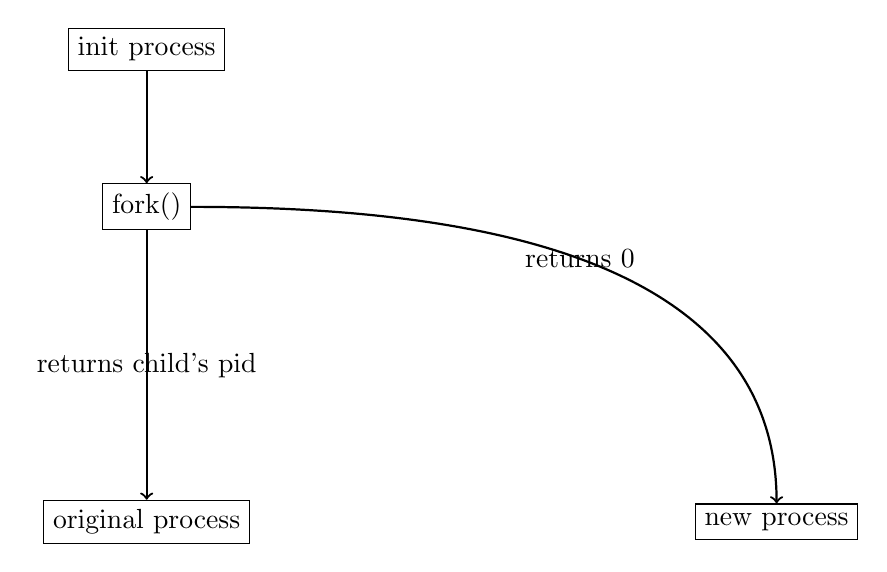
\begin{tikzpicture}
\node (i) [rectangle,draw] at (0,6) {init process};
\node (f) [rectangle,draw] at (0,4) {fork()};
\node (o) [rectangle,draw] at (0,0) {original process};
\node (n) [rectangle,draw] at (8,0) {new process};
\draw [->,thick] (i)--(f) ;

\draw [thick,->] (f) to[out=0,in=90] node{returns 0} (n);
\draw [thick,->] (f) to[out=270,in=90] node{returns child's pid} (o);
\end{tikzpicture}
\end{frame}
\begin{frame}{exec图示}
\begin{tikzpicture}
\node (i) [rectangle,draw] at (0,6) {init process};
\node (f) [rectangle,draw] at (0,4) {exec};
\node (o) [rectangle,draw,dashed] at (0,0) {original process};
\node (n) [rectangle,draw] at (8,0) {new process};
\draw [->,thick] (i)--(f) ;

\draw [thick,->] (f) to[out=0,in=90]  (n);
\draw [dashed,thick,->] (f) to[out=270,in=90] node{X} (o);
\end{tikzpicture}
\end{frame}

\begin{frame}{system图示}
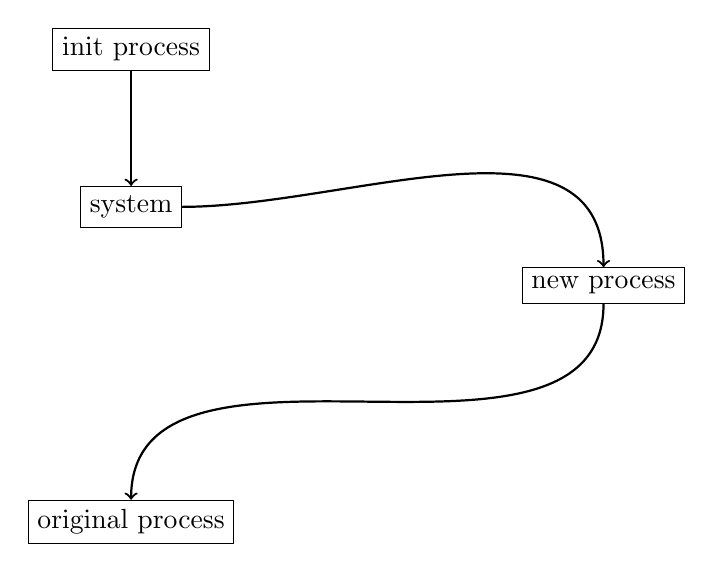
\begin{tikzpicture}
\node (i) [rectangle,draw] at (0,6) {init process};
\node (f) [rectangle,draw] at (0,4) {system};
\node (o) [rectangle,draw] at (0,0) {original process};
\node (n) [rectangle,draw] at (6,3) {new process};
\draw [->,thick] (i)--(f) ;

\draw [thick,->] (f) to[out=0,in=90]  (n);
\draw[thick,->] (n) to[out=270,in=90] (o);
\end{tikzpicture}
\end{frame}


\begin{frame}[fragile]{fork的典型使用方式}
\begin{block}{fork1.c }
\begin{verbatim}
int main(){
 pid_t pid=fork();
 switch(pid){
  case -1:
   printf("error!");
   break;
  case 0:
   printf("I am the child process.\n");
   execlp("/Users/hainingzhang/linux/system1","system1",0);
   break;
  default:
   printf("I am the parent process.\n");
   printf("I want to do something more...\n");
   break		
 } exit(0); }
\end{verbatim}
\end{block}
\end{frame}
\begin{frame}[fragile]{Waiting for a process}
fork了一个新进程之后中,这个新进程就自主的去运行了。但是有些时候父进程想知道子进程的状态,比如,子进程是否结束了?这种情况下可以使用\textcolor{red}{wait}来实现。
\begin{block}{wait}
\begin{verbatim}
#include <sys/wait.h>
pid_t  wait(int *stat_loc);
\end{verbatim}
\end{block}
The wait system call causes a parent process to pause until one of its child processes is stopped.The call returns the PID of the child process.
\end{frame}
\begin{frame}[fragile]{wait}
\begin{block}{fork1.c}
\begin{verbatim}
if(pid!=0){
 int stat;
 pid_t child;
 child=wait(&stat); 
 printf("the child(pid=%d) has finished.\n",child);
 if(WIFEXITED(stat)!=0){
  printf("child exit with code:%d\n",WEXITSTATUS(stat));
 }else{
  printf("child terminated abnormally.\n");
 }
}

\end{verbatim}
\end{block}
\end{frame}
\begin{frame}{Zombie Process}
Using fork to create processes can be very useful, but you must keep track of child processes. \textcolor{red}{When a child process terminates, an association with its parent survives until the parent in turn either terminates normally or calls wait}. The child process entry in the process table is therefore not freed up immediately. Although \textcolor{red}{no longer active}, the child process is still in the system because its exit code needs to be stored in case the parent subsequently calls wait. It \textcolor{red}{becomes what is known as defunct, or a zombie process}.

If the parent then terminates abnormally, the child process automatically gets the process with PID 1 (init) as parent.
\end{frame}
\begin{frame}[fragile]{zombie example I}
\begin{block}{zombie.c}
\begin{verbatim}
void myOut(char * msg, int i);
int main(){
char * message;  pid_t child=fork();
switch(child){
 case -1:
  message="Wrong.";
  myOut(message,1); break;
  case 0:
   message="Child.";
   myOut(message,2); break;
 default:
  message="Parent."; 
  myOut(message,5); break;
  }
}


\end{verbatim}
\end{block}
\end{frame}
\begin{frame}[fragile]{zombie example II}
\begin{block}{output}
\begin{verbatim}$ ./zombie 2>&1 >/dev/null&
[1] 35240
$ ps -al
  UID   PID  PPID     S    TIME CMD
    0 18965   576     Ss  0:00.02 login -pf hainingzhang
  501 18966 18965     S   0:01.62 -bash
  501 35240 18966     S   0:00.01 ./zombie
  501 35241 35240     Z   0:00.00 (zombie)
    0 35243 18966     R+  0:00.00 ps -al
  501 33922 33921     S   0:00.03 -bash
  501 35123 33922     S+  0:00.03 ssh zhanghaining@210.40.16.99
  \end{verbatim}
\end{block}
\end{frame}

%------------------------------------------------
%------------------------------------------------
%\section{Signal}
%\begin{frame}
%\Huge{\centerline{Signal}}
%\end{frame}
%------------------------------------------------
%------------------------------------------------
\begin{frame}{作业}
编写一个程序,要求如下:
\begin{enumerate}
\item
在父进程中fork出一个子进程
\item
在父进程中,每1秒输出一个大写字母:A$\sim$Z
\item
在子进程中,每1秒输出一个小写字母:a$\sim$z
\end{enumerate}
\end{frame}

\begin{frame}
\Huge{\centerline{The End}}
\end{frame}



\section{Appendix}
\begin{frame}
\Huge{\centerline{Appendix}}
\end{frame}
%----------------------------------------------------------------------------------------
\begin{frame}{本课程相关资源下载}
\begin{enumerate}
\item
ppt

\url{https://github.com/gmsft/ppt/tree/master/linux}
\item
实验指导书

\url{https://github.com/gmsft/ppt/tree/master/book/linux}
\end{enumerate}
\end{frame}
\begin{frame}
\frametitle{about man page}
The manual is generally split into eight numbered sections, organized as follows (on Research Unix, BSD, macOS and Linux):
\begin{table}
\begin{tabular}{ll}
\toprule
\textbf{section} & \textbf{description} \\
\midrule
1 & General commands\\
 2 & System calls\\
 3& Library function(C standard library)\\
 4 & Special files(devices) and drivers\\
  5 & File formats and conventions\\
  6  & Games and screensavers\\
   7  & Miscellanea\\
   8   & System administration commands and daemons\\  
\bottomrule
\end{tabular}
\caption{man page}
\end{table}

在终端中运行man read 与 man 2 read ,观察其输出的区别。
\end{frame}

\end{document} 
